\section{Method}

\subsection{Source of data}

For this comparative study the following data sources will be used

\begin{enumerate*}
	\item \acrfull{ac:nibio}
	\item \acrfull{ac:kilden}
	\item \acrfull{ac:met}
\end{enumerate*}

\subsection{Dataset}

The dataset is chosen from four regions in Norway; Innlandet, Vestfold, Trøndelag, and Østfold. From each region are four stations picked:
\begin{table}[h]
	\begin{adjustwidth}{-1in}{-1in}
		\centering
		\begin{tabular}{ccccccccc}
			\hline Region&Name&ID&Drain type&Soile category&Texture&MET name& Latitude&Longdetude\\\hline
			Innlandet&Apelsvoll&11& Selvdrenert&CM& 17&SN11500&60,70024&10,86952\\
			Innlandet& Fåvang&17& Selvdrenert&CM& 15&SN13150&61,45822&10,1872\\
			Innlandet& Ilseng&26& Selvdrenert&PH& 17&SN12180&60,80264&11,20298\\
			Innlandet& Kise&27& Vannmettet&GL& 99&SN12550&60,77324&10,80569\\
			Trøndelag& Kvithamar&57& Vannmettet&ST& 16&SN69150&63,48795&10,87994\\
			Trøndelag& Frosta&15& Selvdrenert&LP& 13&SN69655&63,56502&10,69298\\
			Trøndelag& Mære&34& Selvdrenert&RG& 14&SN71320&63,94244&11,42527\\
			Trøndelag& Rissa&39& Vannmettet&PL& 13&SN71320&63,58569&9,97007\\
			Vestfold& Lier&30& Vannmettet&ST& 16&SN19940&59,79084&10,25962\\
			Vestfold& Sande&42& Vannmettet&ST& 16&SN26990&59,6162&10,22339\\
			Vestfold& Tjølling&50& Selvdrenert&AR& 13&SN27780&59,04641&10,12513\\
			Vestfold& Ramnes&38& Vannmettet&ST& 16&SN27315&59,38081&10,2397\\
			Østfold& Rakkestad&37& Vannmettet&ST& 18&SN3290&59,38824&11,39042\\
			Østfold& Rygge&41& Selvdrenert&AR& 13&SN17380&59,39805&10,75427\\
			Østfold& Tomb&52& Vannmettet&ST& 16&SN17050&59,31893&10,81449\\
			Østfold& Øsaker&118& Vannmettet&ST& 18&SN3370&59,31936&11,04221\\\hline
		\end{tabular}
	\end{adjustwidth}
	\caption[Soil information for each station/w location and MET-ID]{Station information from stations used in this study. The texture class is defined in this article: https://nibio.no/tema/jord/jordkartlegging/jordsmonnkart/dominerende-tekstur-i-overflatesjikt}
\end{table}

All stations are sampled from the date\footnote{Format month-day} 03-01 to 10-31 from 2016 to 2020. The features rain (RR), mean soil temperature at 10cm (TJM10), mean soil temperature at 20cm (TJM20), and air temperature at 2m (TM) are sampled from the LMT database. The soil type, and soil texture is sampled from Kilden from Norwegian Institute of Bioeconomy Research.

\subsubsection{Selection process}
The selection process for finding these station can be compiled into these steps

\begin{enumerate}
	\item Recommendation from Norwegian Institute of Bio-economy Research
	\item \label{list:na_anal}Compute the missing values in the data
	\item Missing values analyse 
	\item Searching LMT database for alternative station candidates if current data is insufficient
	\item If some station was replaced the repeat step \ref{list:na_anal}
\end{enumerate}

\begin{figure}
	\centering
	\includegraphics[width=0.8\linewidth]{"../../results/plots/Plot_test_naive_nan_k17_fTJM20.pdf"}
	\caption[Visual representation of station 17]{Visual representation of missing values at station 17 from 2014 to 2022 at the parameter "TJM20". The left numbers indicated how many hours that are missing and how many of them are shorter than or longer than 5 hours. The yellow markings indicate possible outliers based on the given year, all markings was checked if they were actual outliers. The red colouring indicate missing values in the data (represented in the data with code "NULL").}
	\label{fig:plot-17}
\end{figure}

The plots of stations follow a simple representation where the y-axis represent the year and the x-axis represent the index of the data as all tables are taken from the same period. A circle represent a singluar na values, while a band represent a series of 2 or more missing values. The colours represents the features used in this comperative study. This representation of the missing values will indicate sesonal, and systematic removal of data and give an overall indication of how much data is missing. To get further insight into the data a report is generated in parallel to the plots describing precise date and time of all values and which other parameter values is also missing values in the same period. See appendix \ref{apx:code:dataanal} for the full detail of the report generation and appendix \ref{apx:plots} for na-plots of the station chosen for this study.

\subsubsection{Collection of data}

The method used was a powershell\footnote{Version 7.3.11} script that called the respective institutions servers using the "curl" program\footnote{curl 8.4.0 (Windows) libcurl/8.4.0 Schannel WinIDN} to send an http request for the timeseries starting from 2014 to 2020 in the interval 1 of May to 31 of October. Code for data collection can be viewed in appendix \ref{apx:code:datacollect}. The data is stores as an either a csv file or a json file for easy retrieval and manual control of values.

\subsubsection{Labeling of stations between Nibio and MET}
\begin{table}
	\centering
	\begin{tabular}{r|p{5cm}|}
		FROST & Description\\\hline
		Stations with rain & Requested rain data in millimeters. \\
		Station ID & Sendt a request to LMT for station information using their remote API. \\
		\hline LMT & Description \\\hline
		Meteorological data & Requested soil temperature from 10cm depth, and 20cm depth and air temperature (2m), from 2014-03-01 to 2022-10-31.\\
	\end{tabular}
	\caption[Request to servers about stations]{Description of what was requested from each server (FROST part of \acrshort{ac:met}, \acrshort{ac:nibio}).}
	\label{tab:station_request}
\end{table}

Since Nibio and MET have different names for the same stations one must compile a list that converts Nibio ID to MET ID. This was performed with these requests shown in table \ref{tab:station_request} where ID is the Nibio Id for the given station, Frost.ID is the MET id, ID. latitude is the latitude gathered from Nibio, ID.longitude is the longitude gathered from Nibio. These variables can be swaped out for the relevant station.\todo{Move to caption}

\subsubsection{Storage of data}
The storage of the data is done through two data structures; \gls{gl:hashmap} and \gls{gl:dataframe} from the package pandas. The transformation of data is done with a costume datatype called "DataFileHandler" which is converted to a module for convenience. The keys for the hashmap is chosen by the naming of the data files and the pattern given to the class. To escalete modeling the data will also be exported to a binary file for faster retrieval. \todo{MORE DETAIL}

\begin{figure}
	\centering
	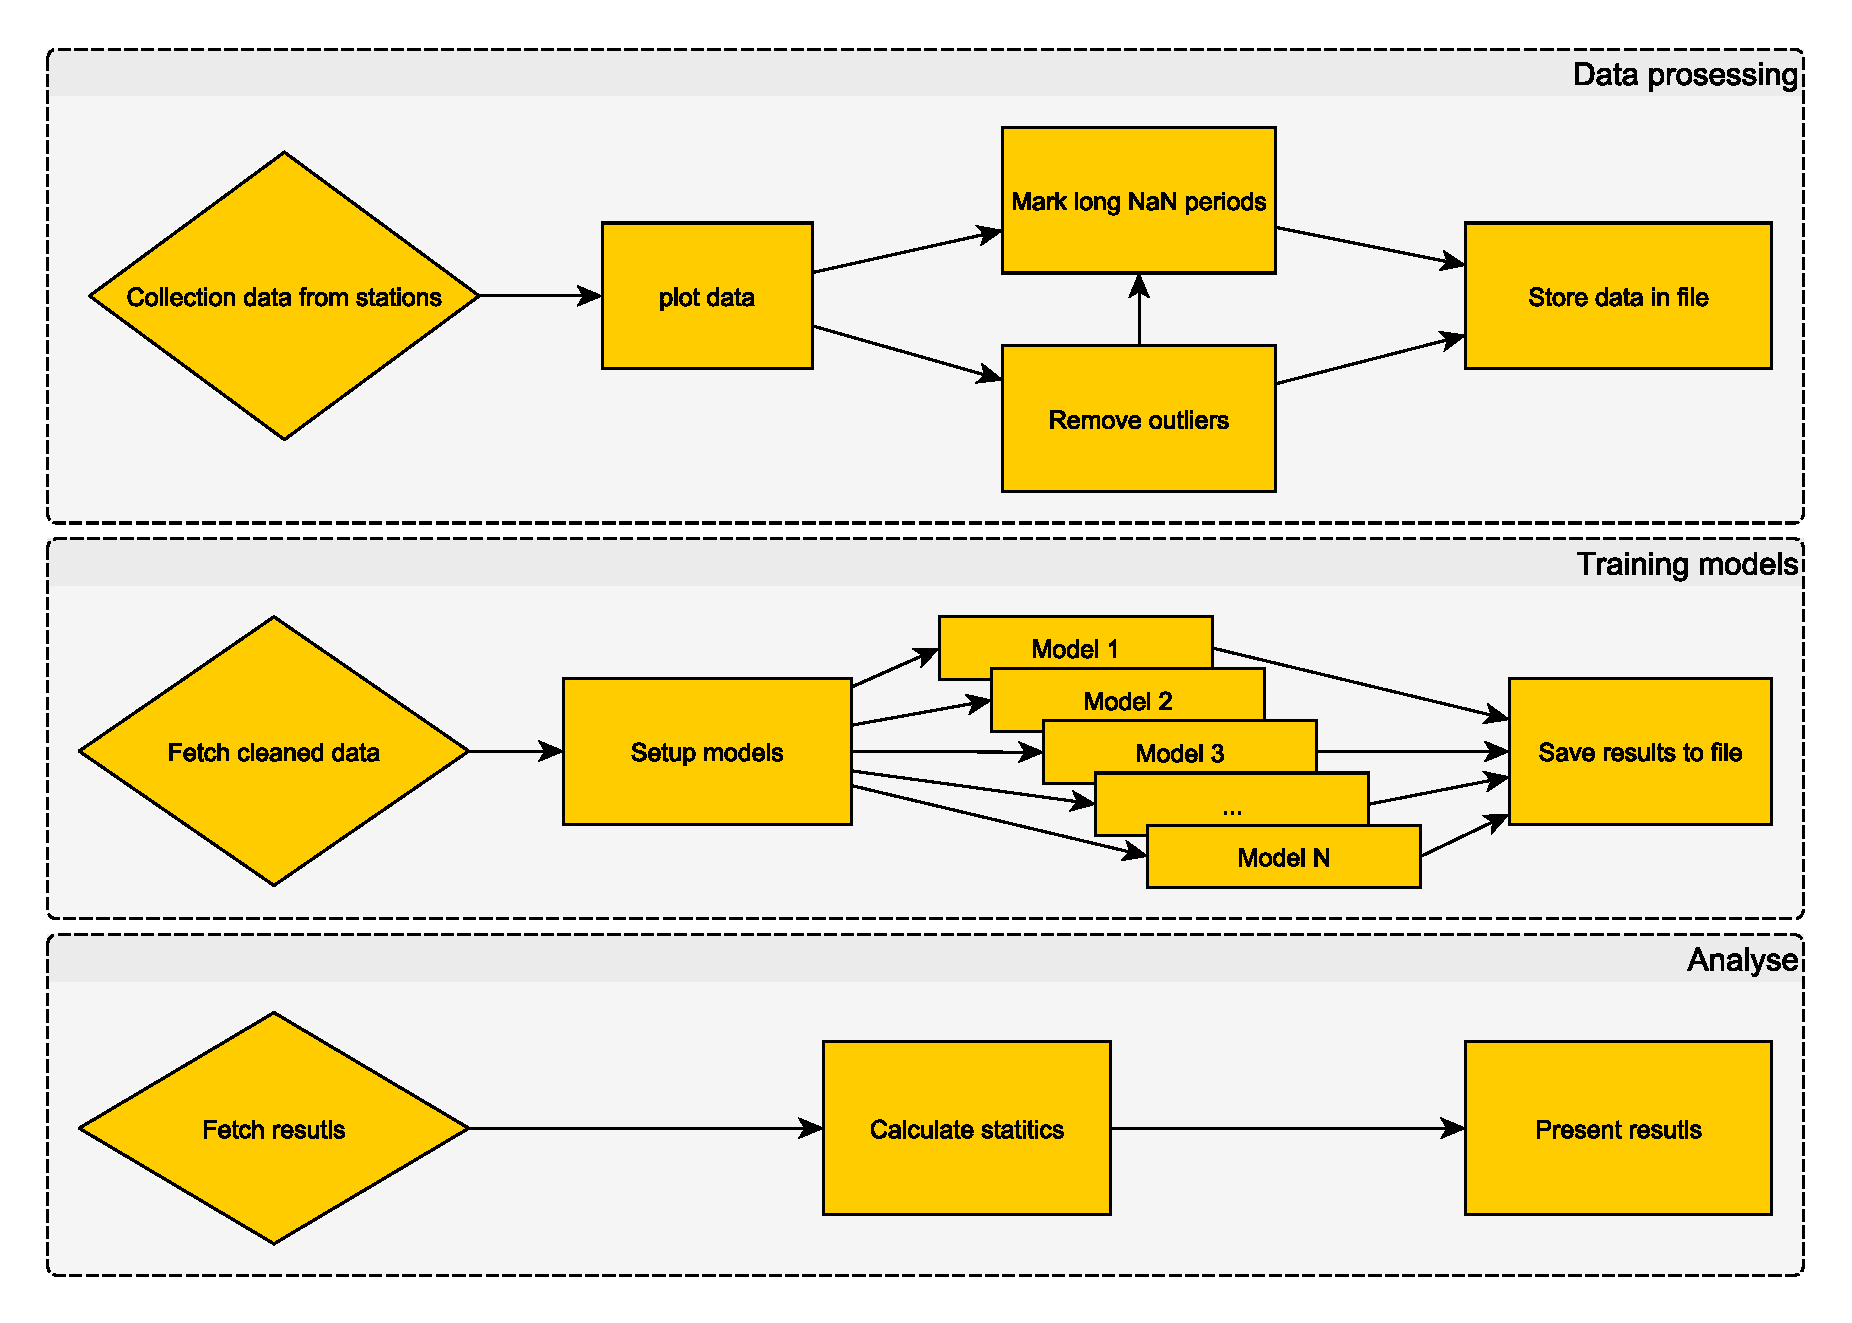
\includegraphics[width=0.7\linewidth]{figures/progress_diagram}
	\caption[Diagram sketching three procedures used in this study.]{A surface level diagram of the methodology.}
	\label{fig:progressdiagram}
\end{figure}\todo{Complete diagram}

\paragraph[Data structure]{Technical overview of custom data structure}
The data structure used to store the data from the different stations is called "DataFileHandler" and stores the data in a tree-structure where indexes are dictated by the filename. It has several built-in functions to assist with data partitioning, and merging of data. This makes it easier to move and store all 846 720 observations from 16 station from all 4 regions\footnote{there are 4 stations per region.}. Further more, the data structure has iteration functions so it is compatible with python's built in loops, and print functions. 

\subsection{Data cleaning and treatment}

To use the data in this study it must be cleaned and treated for training. Though the data has been examined by the supplier, however it still had outliers that needed to be treated before modelling. For this reason several steps and methods is utilized in the prepossessing steps.

\subsubsection{Outlier detection and removal}\todo{Revise so it reflects what you actually do}

Though the data fetched from \acrshort{ac:nibio} is treated and controlled the external data from \acrshort{ac:met} might not be, and this research project incorporated raw, untreated data from \acrshort{ac:nibio} to fill inn missing values.

The method to quickly find obvious outliers was to look at the following condition
$$
	\left|\frac{|\Delta T|-E(|\Delta T|)}{Var(|\Delta T|)}\right|> 4C^\circ
$$\todo{Make more clear}

This condition looks at the absolute difference between consecutive measurements and calculates the z-score for each observation. It is expected that the change in temperature can't be too rapid. Further methods used to highlight potential outliers is 

\begin{figure}[h]
	\centering
	\definecolor{zzttqq}{rgb}{0.6,0.2,0.}
	\definecolor{REDDD}{rgb}{0.8,0.5,0.2}
	\definecolor{ududff}{rgb}{0.30196078431372547,0.30196078431372547,1.}
	\begin{tikzpicture}[line cap=round,line join=round,>=triangle 45,x=1.0cm,y=1.0cm]
		\begin{axis}[
			x=1.0cm,y=1.0cm,
			axis lines=middle,
			ymajorgrids=true,
			xmajorgrids=true,
			xmin=-0.5,
			xmax=3.5,
			ymin=-0.5,
			ymax=2.5,
			xtick={-0.0,1.0,...,3.0},
			ytick={-0.0,1.0,...,2.0},]
			\clip(-0.5,-0.5) rectangle (3.5,2.5);
			\draw [line width=2.pt,dash pattern=on 1pt off 1pt] (1.04,1.02)-- (3.04,0.02);
			\draw [line width=2.pt] (1.04,1.02)-- (2.04,2.02);
			\draw [line width=2.pt] (2.04,2.02)-- (3.04,0.02);
			\begin{scriptsize}
				\draw [fill=ududff] (1.04,1.02) circle (2.5pt);
				\draw[color=ududff] (1.18,1.39) node {$A$};
				\draw [fill=ududff] (3.04,0.02) circle (1.5pt);
				\draw[color=ududff] (3.18,0.31) node {$B$};
				\draw [fill=ududff] (2.04,2.02) circle (1.5pt);
				\draw[color=ududff] (2.18,2.31) node {$C$};
				\draw [fill=zzttqq] (2.,0.54) circle (2.5pt);
				\draw [color=REDDD,dashed] (2.,0.54) circle (0.5);
				\draw[color=zzttqq] (2.14,0.91) node {$C^*$};
			\end{scriptsize}
		\end{axis}
	\end{tikzpicture}
	\caption[Simple Interpolation outlier detection]{An simple outlier detection method utilizing a simple line to estimate where the expected point ($C^*$) is supposed to be. If observed point C falls outside the tolerance level (red dotted circle) then it is marked as an outlier.}
\end{figure}

\subsubsection{Missing value imputation}

The data has missing values, in particular during early Fall when there were sub-zero temperatures meaning any rain measurements done during this period would have unpredictable fluctuations since at negative temperatures water can freeze, get clogged up with residual bio-material from the surrounding area \todo{Rewrite this part to reflect what is going on}. When interpolation the values the method chosen is a linear interpolation with a maximum period to interpoate is 5 hours for Soil temperatures, and 3 hours for air temperatures. The resoning for this is that the soil temperatures are more reliable makeing it safer to interpolate without loosing too much information, while air temperaturses has a higher variance makeing it more difficult to interpolate without cutting values.

\subsection{Setup of models}\todo{In general, write more on all subsections}

The models are set up in according to the relevant paper the model is fetched from, alternatively reuse the code made by the author. When importing the data to the model there will be modifying to the original code to facilitate for the model as far as it goes. Any modifications will be in the appendix under section \ref{apx:code}. For the convenience of the reader all code is using the sklearn estimator class to make all the models discuses in this study more user friendly and compatible with sklearns other functions. The details of the models will be discussed in section \ref{sec:theory}, this section discusses the setup and implementation of the models.\footnote{Caution to the reader; The code used was run on the Linux subsystem (Debian) on windows due to the fact that the current version of tensorflow can't run on Windows.}

\subsubsection{Basic Linear model}

The linear model (section \ref{sec:theory:linreg}) utilises in the study is created from the python model sklearn (or scikit-learn according to pythons package manager). The model is setup with standard parameters, and the data is fed into the model without scaling with fitted intercept coefficient. 

\subsubsection{Plauborg}

The Plauborg regression will be formulated as a linear regression problem so that the LinearRegression function in the Sci-kit module can be used. For the parameters used in the paper\cite{plauborg_simple_2002} the F function defined in section \ref{sec:theory:pluborg} will be formulated with loops to give rise 3 more parameters for fine-tuning the model. Nan-values generated from the procedure get replaced with 0, since the data fed to the model is segnificantly larger than 10h (the minimum for the training is 24h).

\subsubsection{LSTM}\todo{rewrite or possibaly move}

Long Short-Term Memory (LSTM) networks are a specialized type of Recurrent Neural Network (RNN) designed to handle long-term dependencies in sequential data. Unlike regular RNNs, which often suffer from vanishing gradient problems, LSTMs utilize a more complex cell structure that allows them to capture long-term dependencies more effectively.

\begin{itemize}
	\item \textbf{Input Gate (it​)}:
	$ a_i = \sigma(W_{xi} \cdot X_t + W_{hi} \cdot H_{t-1} + b_i) $
	\item \textbf{Forget Gate ($f_t$)}:
	\[ a_f = \sigma(W_{xf} \cdot X_t + W_{hf} \cdot H_{t-1} + b_f) \]
	
	\item \textbf{Cell State Update ($\tilde{C}_t$)}:
	\[ \tilde{C}_t = \tanh(W_{xc} \cdot X_t + W_{hc} \cdot H_{t-1} + b_c) \]
	
	\item \textbf{New Cell State ($C_t$)}:
	\[ C_t = f_t \cdot C_{t-1} + i_t \cdot \tilde{C}_t \]
	
	\item \textbf{Output Gate ($o_t$)}:
	\[ a_o = \sigma(W_{xo} \cdot X_t + W_{ho} \cdot H_{t-1} + b_o) \]
	
	\item \textbf{Hidden State ($H_t$)}:
	\[ H_t = o_t \cdot \tanh(C_t) \]
	
\end{itemize}
Where:
\begin{itemize}
	\item[\(X_t\)] represents the input at time step (t).
	\item[\(H_{t-1}\)]  is the hidden state from the previous time step.
	\item[\(W\) and \(b\)]  are weight matrices and bias terms.
	\item[\(\sigma\)]  denotes the sigmoid activation function
	\item[\(\tanh\)]  represents the hyperbolic tangent activation function.
\end{itemize}

LSTMs have proven effective in various tasks such as natural language processing, speech recognition, and time series prediction. They provide a powerful mechanism for modeling sequential data while mitigating the vanishing gradient problem commonly encountered in vanilla RNNs.

\subsubsection{BiLSTM}\todo{rewrite}

Bidirectional Long Short-Term Memory (BiLSTM) networks enhance traditional LSTMs by considering context from both forward and backward directions. Here’s how they work:

BiLSTMs consist of two LSTM layers operating simultaneously:

- The forward LSTM processes the input sequence from the beginning to the end.
- The backward LSTM processes the input sequence from the end to the beginning. By combining the outputs of these two LSTMs, BiLSTMs effectively capture information from both past and future context.
- This context expansion is particularly useful in tasks where context matters in both directions:

Natural Language Processing (NLP): BiLSTMs excel in tasks like part-of-speech tagging, named entity recognition, and sentiment analysis.
- Speech Recognition: Capturing context from both sides of an audio sequence improves accuracy.
- Time Series Prediction: BiLSTMs enhance predictions by leveraging past and future data points.
- Mathematically, the final hidden state of the BiLSTM at time step (t) is the concatenation of the forward and backward LSTM hidden states: \[ H_t = [H_t^{(f)}, H_t^{(b)}] \] The resulting output can be used for downstream tasks such as classification, regression, or sequence labeling.

Information from earlier timesteps is important to say something about current timesteps, same can be said about the other time direction. To get the best of both direction one can use a bidirectional LSTM (BiLSTM) to combine the information from both approches. To make one of the models read the data backwards the model pipeline reverses the data and trains on that. A visualiation of this can be shown in the first layer in figure \ref{fig:bilstm}.

\subsubsection{Modified BiLSTM}

To investigate the posssibility of RNN a more complex model was developed to see if the introduction of more layers would improve the accuratsy of the base model. 

\begin{figure}[H]
	\centering
	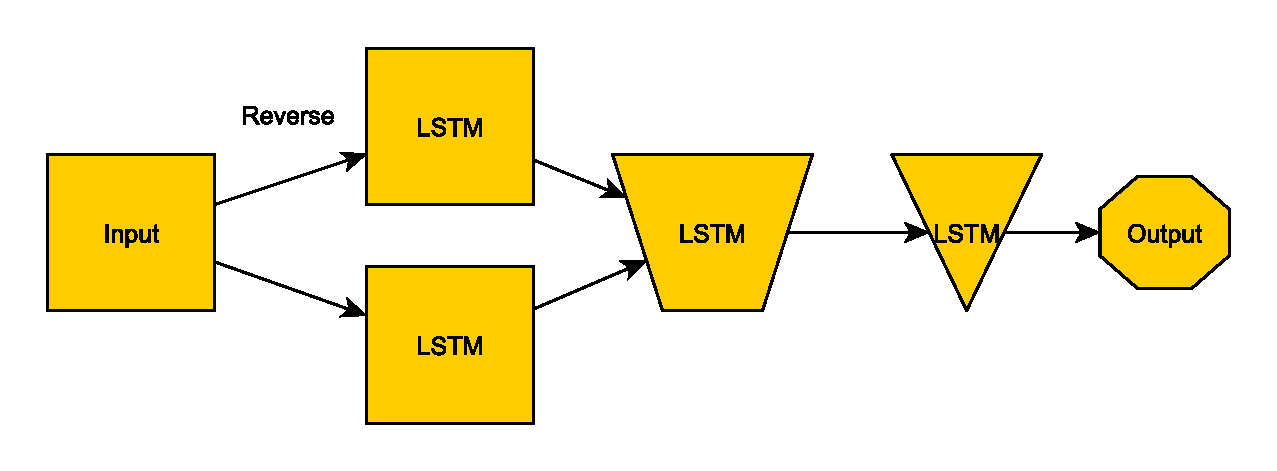
\includegraphics[width=0.7\linewidth]{figures/BiLSTM}
	\caption[modified BiLSTM overview]{Simple diagram of the structure of the BiLSTM. The data from the input layer gets duplicated and passed to two LSTM's where one of them get the data in reverse. When both models have trained on the data they gets concatenated and passed to another LSTM that has half of the units as output. The final LSTM has a single cell as output leaving a single value as the prediction.}
	\label{fig:bilstm}
\end{figure}\todo{Complete caption, and improve figure}

Soil temperatures depend on earlier timestamps, so to make accurate predictions, it's essential to include temperature data from $t, t-1, \dots, t-k$. Evaluating the data both forwards and backwards helps identify features that are noticeable in specific directions. The BiLSTM model, implemented using TensorFlow's Keras module, consists of three layers:\todo{EXPAND}

\begin{itemize}
	\item A Bidirectional LSTM layer for feature extraction.
	\item A regular LSTM layer to condense information with a tanh activation function
	\item An LSTM layer for prediction with a tanh activation function
\end{itemize}

The activation functions used are hyperbolic tangent and sigmoid. The output layer employs the identity function ($f(x) = x$). The hidden layer has half as many recurrent cells as the input layer, and the output layer condenses the hidden layer's output to a single value. For more details, refer to Figure \ref{fig:bilstm} and Table \ref{tab:subtab:BiLSTM_params}.

\begin{table}
	\centering
	\begin{subtable}[t]{0.45\textwidth}
		\begin{tabular}{l|c}
			Parameter name & Range \\\hline\hline
			Epochs & [4,8] \\
			Units & \(\{2^6,2^7,2^8\}\) \\
			Lag time & \(12i\) for \(i \in [1,14]\)
		\end{tabular}
		\caption[Parameter space for modified BiLSTM]{The search space for the modified BiLSTM model. The units define the number of LSTM cells used in the LSTM output. The lag time specifies how many hours the model will take into account when predicting soil temperature. The square brackets indicate an interval including endpoints, while the curly brackets indicate a list of elements.}
		\label{tab:subtab:BiLSTM_params}
	\end{subtable}
	\hfill
	\begin{subtable}[t]{0.45\textwidth}
		\begin{tabular}{l|c}
			Parameter name & Range \\\hline\hline
			Sine terms & [1,10] \\
			Cosine terms & [1,10] \\
			Lag time & [1,14]
		\end{tabular}
		\caption[Parameter space for Plauborg]{The search space for the Plauborg model. The square brackets indicate an interval including endpoints. The "Lag time" indicated the number of time-steps before current time-steps do the model include ($t_{-1},t_{-2},\dots$)}
		\label{tab:subtab:plauborg_params}
	\end{subtable}
	\begin{subtable}[t]{0.45\textwidth}
		\begin{tabular}{l|c}
			Parameter name & Range \\\hline\hline
			Epochs & [4,10]\\
			Lead time & $\{24*n|n\in[1,7]\}$\\
		\end{tabular}
		\caption[Parameter space for BiLSTM and LSTM]{Parameter space for both LSTM and BiLSTM. The square brackets indicate an interval including endpoints. The "Lag time" indicated the number of time-steps before current time-steps do the model include ($t_{-1},t_{-2},\dots$)}
	\end{subtable}
	\caption{Parameter search space for the different deep learning models}
	\label{tab:model_params}
\end{table}

This model is an extention of \citetitle{li_modeling_2020}\cite{li_modeling_2020} written by \citeauthor{li_modeling_2020}. 

\subsection{Metrics}\label{sec:method:metric}

The metrics used in this study are

\begin{itemize*}
	\item \acrfull{ac:rmse}
	\item \acrfull{ac:mae}
	\item \acrfull{ac:r2}
	\item bias
	\item \acrfull{ac:kappa}
	\item digit sensitivity
\end{itemize*}

Soil temperatur as a differnet behavor than air temperature since energy (temperature) though the soil gets dampen and delayed. Since the data used in this study has outliers that was not cought during datatreatment, which has been addresed, the author of this study desided to include two more metrics that are not usually included in the evaluation; The log condition number, and digit sensitivity. Both metrics are based on the calculation of the condition number defined as 

\begin{equation}\label{eq:kappa}
\kappa = \lim\limits_{\varepsilon \to 0^+} \sup\limits_{|\partial x|\leq\varepsilon}  \frac{\left|f(x+\partial x) - f(x)\right|}{|f(x)|}*\frac{|x|}{|\partial x|} 
\end{equation}

This is not feasible to calculate since infinite calculations with infinitesimal numbers is not possible as per $\today$ for simulation approach\footnote{This calculation is possible for some models, for instance linear regression models when converted to the form $A\vec{\beta} = \vec{y}$.}. Therefore this paper uses algorithm \ref{alg:cond_num} to approximate $\kappa$ for all the models.

\begin{algorithm}[H]
	\SetAlgoLined
	\KwData{ Data }
	\KwResult{log($\kappa$)}
	Let $\kappa_f$ be the function \ref{eq:kappa}\;
	$\kappa\gets 0$\;
	\For{$i \in {1 \dots |Data|}$}{
		$\partial x \gets \mathcal{U}_{[-\sqrt{\varepsilon/|Data|},\sqrt{\varepsilon/|Data|}]}$\;
		$k \gets$ calculate with $\kappa_f$ from $x$ and $x+\partial x$\;
		\If{k > $\kappa$}{$\kappa \gets k$\;}
	}
	\Return{$\kappa$}
	\caption[Randommised $\kappa$ algorithm]{Method for calculating $\kappa$. $\mathcal{U}$ is a uniform random distrebution in a range.}
	\label{alg:cond_num}
\end{algorithm}

The digit sensitivity is included to give an intitive understanding of $\kappa$ and is computed simply as $\log_e(\kappa)+1$. This number tells us the significant digit generated from the model. If the number is less than 0 then its the ith digit after the decimal point.

For the rest of the metrics, they are defined as follows
\begin{itemize}
	\item \gls{ac:rmse} = $\sqrt{\frac{\sum (y_{\text{pred}} - y_{\text{truth}})^2}{n}}$
	\item \gls{ac:mae} = $\frac{\sum \left| y_{\text{pred}} - y_{\text{truth}}\right|}{n}$
	\item bias = $\frac{\sum ( y_{\text{pred}} - y_{\text{truth}})}{n}$
	\item \gls{ac:r2} = $1-\frac{\sum (y_{\text{pred}} - y_{\text{truth}})^2}{\sum (y_{\text{pred}} - \vec{y})^2}$
\end{itemize}

Where $\vec{y}$ is the mean of the target, $y_{\text{pred}}$ is the predicted data, and $y_{\text{truth}}$ is the observed soil temperature.

\subsubsection{Model training}

The models get trained on air temperature, however the precise input for each model is not the same for all. The features used for each model are described in table \ref{tab:model_params} and their transformation in table \ref{tab:model_trans}.

The models get a sample of the training data at the time due to the size and the amount for missing data (for example figure \ref{fig:plot-17}) The algorithm used to fetch reliable indexes are demonstrated at algorithm \ref{alg:find_non_nan_ranges_abstract}.

\begin{algorithm}
	\caption{Find Non-NaN Ranges (Abstract)}
	\label{alg:find_non_nan_ranges_abstract}
	\SetKwFunction{FindNonNaNRanges}{FindNonNaNRanges}
	\SetKwInOut{Input}{Input}
	\SetKwInOut{Output}{Output}
	
	\Input{Input data $\text{data}$}
	\Output{List of tuples: $\text{ranges}$}
	
	\BlankLine
	\SetKwData{StartIdx}{start}
	\SetKwData{NonNaNRanges}{ranges}
	\SetKwData{Item}{item}
	
	\FindNonNaNRanges{$\text{data}$}{
		$\NonNaNRanges \gets$ empty list\;
		$\StartIdx \gets$ None\;
		
		\For{$\Item \text{ in } \text{data}$}{
			\If{$\Item is not Nan$}{
				\If{$\StartIdx \text{ is None}$}{
					$\StartIdx \gets \Item$\;
				}
			}
			\Else{
				\If{$\StartIdx \text{ is not None}$}{
					Add ($\StartIdx$, $\Item$ index - 1) to $\NonNaNRanges$\;
					$\StartIdx \gets$ None\;
				}
			}
		}
		\If{$\StartIdx \text{ is not None}$}{
			Add ($\StartIdx$, Last index) to $\NonNaNRanges$\;
		}
		\Return $\NonNaNRanges$\;
	}
\end{algorithm}


\begin{table}[H]
	\centering
	\begin{tabular}{|r|c| p{6cm}|}
		\hline model name & features & transformations \\\hline\hline
		Linear regression & TM & Time get translated to hours by taking the day since new year and multiplying by 24 for then add the hour part. \\\hline
		Plauborg & Time, TM & Time get translated in two way; the current day since new year if looking at daily values, and hours since new year if looking at hourly predictions. When converting TM to daily values the hourly data get averaged. \\\hline
		BiLSTM &Time, TM& Time get translated to hours since new year.\\\hline
	\end{tabular}
	\caption[Model parameters]{Parameters used for predicting soil temperatures at depth 10cm and 20cm.}
	\label{tab:model_trans}
\end{table}


